% Chapter 1

%\chapter{Curriculum Vitae} % Main chapter title

%\label{CV} % For referencing the chapter elsewhere, use \ref{Chapter1} 

% \lhead{Chapter 1. \emph{Introduction}} % This is for the header on each page - perhaps a shortened title

\graphicspath{{./Pictures/}}

%----------------------------------------------------------------------------------------

\newpage
\pagestyle{plain}
\vspace{-9cm}

\LARGE
\textbf{Curriculum Vitae}

\bigskip
\bigskip
\Large
\textbf{Personal Details}
\noindent\rule[0mm]{\linewidth}{2pt}

\normalsize
\begin{tabbing}
First Name \hspace*{2.4cm} \= Raphael \\
Surname \> Wolfisberg \\
Date of Birth \> 14. May 1988 \\
Nationality \> Swiss \\
\medskip
E-mail \> raphael.w@hotmail.com \\
Mobile \> +41 79 837 19 62 
\end{tabbing}

\vspace{-4.4cm}
\begin{flushright}
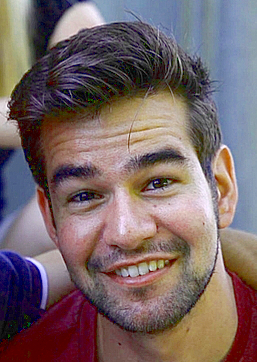
\includegraphics[scale=0.35]{Rafa} \\[1cm]
\end{flushright}


\vspace{-0.8cm}
\Large
\textbf{Education}
\noindent\rule[0mm]{\linewidth}{2pt}

\normalsize
\begin{tabbing}
Mar. 2012 - present \hspace*{0.9cm} \= Ph.D. at the Department of Chemistry and Biochemistry (DCB) \\ 
\> University of Bern, Switzerland  \\
\> Title of the Ph.D. thesis: ``Characterization of the prelytic
active \\ 
\> egress of a non-enveloped virus.'' \\
\> Supervisors: Dr. Carlos Ros and Prof. Dr. Christoph Kempf \\ [0.3cm]
Oct. - Dec. 2013 \> Scientific exchange at Centro de Biología Molecular Severo Ochoa \\
\> Universidad Autónoma de Madrid \\
\> Collaboration with Prof. Dr. José María Almendral del Río \\ [0.3cm]
Sept. 2010 - Jan. 2012 \> Master of Science (MSc) in Chemistry and Molecular Science \\
\> DCB, University of Bern, Switzerland  \\
\> Title of the master thesis: ``Changing the surface of human \\ \> parvovirus B19'' \\
\> Supervisors: Dr. Carlos Ros and Prof. Dr. Christoph Kempf \\ [0.3cm]
Sept. 2007 - Aug. 2010 \> Bachelor of Science (BSc) in Chemistry or Biochemistry \\
\> DCB, University of Bern, Switzerland  \\
\> Title of the bachelor thesis: ``Die Suche nach dem NMD \\
\> Mechanismus in \textit{Trypanosoma brucei}.'' \\
\> Supervisor: Prof. Dr. André Schneider \\ [0.3cm]
Aug. 2003 - Aug. 2007 \> Grammar school at the Kantonsschule Reussbühl, Lucerne \\
\> Main subjects: physics and applied mathematics

\end{tabbing}


\Large
\textbf{Skills}
\noindent\rule[0mm]{\linewidth}{2pt}

\normalsize
\begin{tabbing}
Languages \hspace{1cm} \= German \hspace{1cm} \= Mother tongue \\
\> English \> Advanced\\
\> French \> Intermediate \\
\> Spanish \> Basics \\
\end{tabbing}